\hypertarget{architecture}{%
\section{Outcomes}\label{sec:architecture}}

The platform was initially deployed in a 6-month pilot phase, where digital twins were created for 22 instrumented bridges in the Caltrans inventory (see \cref{tab:pilots}). In this period, real-time monitoring was performed on the \emph{Hayward Hwy 580-238 Interchange} (CSMIP station \texttt{CE58658}), while the remaining 21 bridges where studied using preexisting records.
Following the success of this trial deployment, development of the platform was resumed with future work expected to expand its coverage of the California highway network.

% Structural vibration sensing and data streaming in California has seen technological developments and investments in recent years. To help monitor the state transportation network, acceleration response records are streamed from discrete locations on highway bridges that are at risk of structural damage or play a key role as recovery routes or lifelines. An ongoing research question is how to best utilize these data to monitor the health of the bridges.

% A complete framework is being developed that allows advanced state-of-the-art methodologies from disciplines like monitoring, assessment, and identification to be linked together in new, and exciting ways. 
% Considerable time and effort has been put into ensuring that the design of the framework is (1) able to remain relevant as progress continues to be made in these fields, and (2) provides a connection between these fields that is able to facilitate new and useful conclusions. Because of the novelty provided by this unique arrangement of tools, the \BRACE{} project sits at a vantage point from which several new possibilities exist for reaching new understandings in the interdisciplinary realm of seismic structural health monitoring.


\subsection{IRiE}
The \emph{infrastructure resilience engine}, \IRIE{}, is a framework for supporting dynamic web applications.
It integrates high-fidelity physics-based modeling of individual assets with real-time accelerometer data streamed from sensors installed on these assets.
The framework provides a link between:
\begin{enumerate}
    \tightlist
    \item Decision-makers who bear the responsibility for public safety and need to make informed decisions about infrastructure.
    \item Practicing engineers who understand the structural mechanics and are equipped to develop prediction models that can accurately forecast the behavior of structures under various conditions.
    \item Researchers or specialists in the field of structural health monitoring who are actively studying and developing new metrics for health assessment.
\end{enumerate}

%
\begin{table} %[h!]
\centering
    \caption{Bridges included in the pilot study for the \BRACE{} platform.}
\begin{tabular}{lllrrr}
\toprule
  \textbf{CESMD} & \textbf{Year}\footnote{Year of initial instrumentation.} & \textbf{Name} & \textbf{Events} & \textbf{Sensors}  & \textbf{Predictors} \\
    \midrule
    \texttt{CE13705} & 1994 & Corona - I15/Hwy91 Interchange Bridge       &   3  &   9 & 6  \\ % &    \\
    \texttt{CE13795} & 1999 & Capistrano Beach - I5/Via Calif. Bridge     &   5  &  12 & 3  \\ % & 5  \\
    \texttt{CE14406} & 1981 & Los Angeles - Vincent Thomas Bridge         &   7  &  26 & 4  \\ % & 7  \\
    \texttt{CE24694} & 1995 & Sylmar - I5/14 Interchange Bridge           &   2  &  42 & 2  \\ % & 2  \\
    \texttt{CE24704} & 1994 & Los Angeles - I10/La Cienega Bridge         &   5  &  15 & 3  \\ % & 5  \\
    \texttt{CE24706} & 1994 & Palmdale - Hwy 14/Barrel Springs Bridge     &   6  &  12 & 3  \\ % & 6  \\
    \texttt{CE24775} & 1998 & Grapevine - I5/Lebec Rd Bridge              &   7  &  16 & 3  \\ % & 6  \\
    \texttt{CE33742} & 1996 & Ridgecrest - Hwy 395/Brown Road Bridge      &   5  &   9 & 3  \\ % & 5  \\
    \texttt{CE47315} & 1977 & San Juan Bautista - Hwy 101/156 Overpass    &  10  &  15 & 3  \\ % & 10  \\
    \texttt{CE68184} & 2002 & Vallejo - Carquinez/I80 East Bridge         &   3  &  58 & 2  \\ % \\
    \texttt{CE68185} & 2004 & Vallejo - Carquinez/I80 West Bridge         &   5  & 103 & 5  \\ % \\
    \texttt{CE79421} & 2009 & Leggett - Hwy 101/Confusion Hill Bridge     &   5  &  24 & 6  \\ % \\
    \texttt{CE89686} & 1996 & Eureka - Samoa Channel Bridge               &  18  &  27 & 4  \\ % \\
    \texttt{CE89708} & 1995 & Arcata - Hwy 101/Murray Road Bridge         &   7  &  12 & 6  \\ % \\
    \texttt{CE89735} & 1996 & Eureka - Middle Channel Bridge              &  14  &   9 & 3  \\ % \\
    \texttt{CE89736} & 1996 & Eureka - Eureka Channel Bridge              &  13  &  12 & 4  \\ % \\
    \texttt{CE89973} & 2001 & Rio Dell - Hwy 101/Eel River Bridge         &  44  &  18 & 3  \\ % \\
    \texttt{CE23631} & 2001 & San Bernardino - I10/215 Interchange        &   9  &  18 & 4  \\ % & 9  \\
    \texttt{CE54730} & 1995 & Lake Crowley - Hwy 395 Bridge               &   5  &   9 & 6  \\ % \\
    \texttt{CE89324} & 1977 & Rio Dell - Hwy 101/Painter St. Overcrossing &  31  &  20 & 6  \\ % \\
    \texttt{CE01336} & 1978 & Hwy8/Meloland Overpass                      &  13  &  32 & 7  \\ % & 13 \\
    \texttt{CE58658} & 1993 & Hayward Hwy 580-238 Interchange             &  62  &  20 & 7  \\ % \\
\midrule
\textbf{Total} & & & 279 & 518 & 93 \\
\bottomrule
\end{tabular}
\label{tab:pilots}
\end{table}

The implementation of the \BRACE{} platform is organized into four distinct modules. Each module implements the fundamental abstractions on the platform and has exclusive control over various tables in the database. % (\cref{fig:database}). 
The remainder of this section will detail this architecture, with a particular focus on the encapsulation provided by these modules and how they interact with each other.
%
To this end we consider three key web pages generated by the platform which exemplify the merits of the abstract framework developed in \cref{sec:framework} (\cref{fig:interface}):
\begin{enumerate}
\tightlist
    \item The \emph{dashboard} renders a high-level snapshot of the bridges that are managed by the platform and available for the decision-maker  (\cref{fig:interface} a).
    \item An \emph{asset page} provides a detailed profile of the physical asset with it's unique vulnerabilities and metadata (\cref{fig:interface} b), as well as a record of all existing evaluations (\cref{fig:interface} c).
    \item An \emph{evaluation page} is a report on the health of an asset, generated in response to an \gls{event} (\cref{fig:interface} d). 
\end{enumerate}
%
\begin{figure}
    \centering
    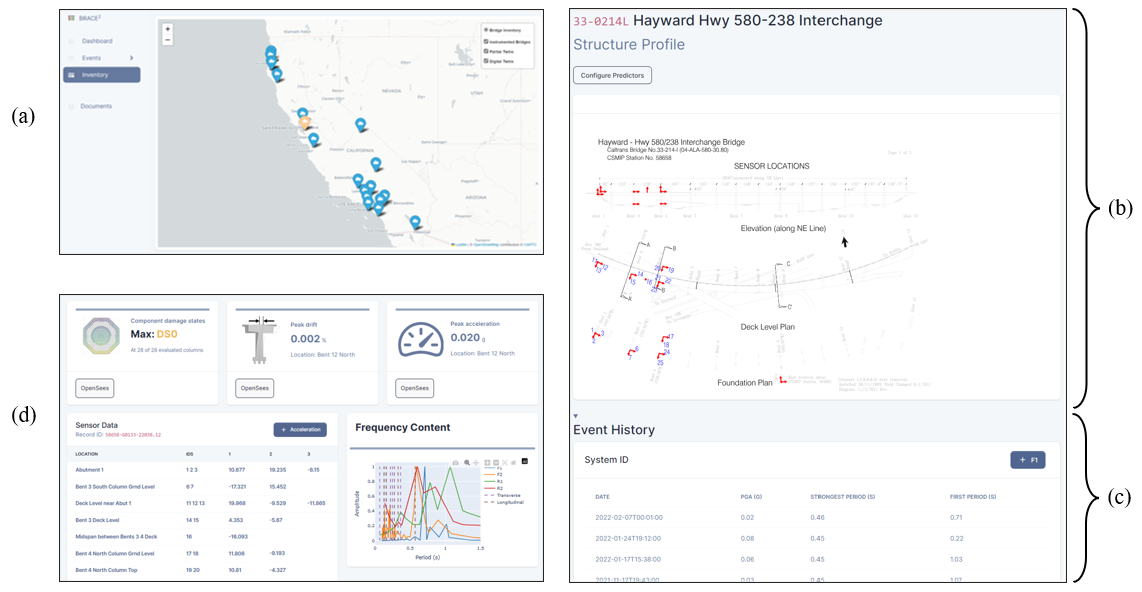
\includegraphics[width=\textwidth]{Body/Irie/Figures/interface.png}
    \caption{Pages from the interface of the \BRACE{} platform: the dashboard (a), an asset page (b) and (c), and an evaluation page (d).}
    \label{fig:interface}
\end{figure}
%

% Implementing a digital twin framework for public infrastructure poses several unique challenges. The platform must facilitate cooperation between several distinct government entities. 
% Data is generally of poorer quality.

% The first phase of the \BRACE{} project involved a full-scale deployment which included a total of \textbf{22} bridges in California, with particular focus on the \emph{route 580/238 separation structure} (Caltrans bridge No. \texttt{33-0214L}).
% These assets are further discussed in \cite{chern2024crosssectional} in the context of \glspl{predictor-t2}.


\subsubsection{The \texttt{inventory} Module}\label{sec:inventory-module}

On the \BRACE{} platform, an \gls{asset} is identified by its FHWA structure ID.

The \texttt{inventory} module is central to the identity of the digital twin. It implements the representation of an \gls{asset} and is primarily concerned with the creation and management of entries in the \texttt{Asset} database table. %(\cref{fig:database}). 
To ensure that an \texttt{Asset} entry can collect all \texttt{Predictor} entries associated with it, the \texttt{inventory} module imports the \texttt{prediction} module (see \cref{sec:prediction-module}).

To incorporate the structural details mentioned in \cref{sec:assets} into the decision-making process, the platform represents assets with a personalized structure profile (\cref{fig:interface} b and c). 
This profile has been designed to integrate seamlessly with the Federal Highway Administration’s National Bridge Inventory, ensuring that all relevant data is readily available.

% The \texttt{inventory} module is responsible for generating inventory pages.

\subsubsection{The \texttt{prediction} Module}\label{sec:prediction-module}
%
The \texttt{prediction} module implements the predictor and metric abstractions. Its responsibilities include management of the \texttt{Predictor} database table and the dispatching of predictor procedures.

\paragraph{Database Management}

The \texttt{Predictor} table serves as a repository for the configurations of the predictors that are invoked to populate the \texttt{Evaluation} entries for a specific \texttt{Asset}. This feature aligns with the objective of creating a dynamic software model that reflects the physical state of a structure, as it allows for the seamless integration of various predictors into the platform.

\paragraph{Procedure Dispatch}

The dispatching of predictors is managed by the \texttt{prediction.predictors} submodule, which implements the abstract \texttt{PredictorDaemon} class and its subclasses. These classes abstract away the implementation details of various predictors, providing a unified interface for their dispatch.

Predictors are invoked as subprocesses, and communication is performed over standard input and standard output streams \citep{silberschatz2018operating}. 
This design ensures efficient resource utilization and allows for the concurrent execution of multiple predictors. 
To facilitate this communication, two protocols have been developed, one for each type of predictor (Type I and Type II). 
The protocols rely on JSON-encoded messaging in a manner that is compatible with frameworks like  \cite{deierlein2020cloudenabled,deierlein2021state}.  

The flexibility afforded by this design has made it possible to integrate a wide variety of scientific computing tools into the platform to be used as predictors. These include the \texttt{mdof} Python library for system identification \citep{chern2024mdof}, the OpenSees Tcl interpreter for nonlinear structural analysis \citep{mckenna1997object}, and the new experimental OpenSeesRT library \citep{perez2024xara}, a redesigned and optimized frontend to the core OpenSees framework which has been redesigned to facilitate model updating and machine learning tasks.
% A pilot study for this class of prediction has been carried out for the route 580/238 separation structure (Caltrans bridge number \texttt{33-0214L}). This is presented in \cite{perez2024brace2}.

The \texttt{PredictorDaemon} class also plays a crucial role in resource management. 
By providing an abstract interface for dispatching predictors, it allows the \texttt{EvaluationDaemon} class of the \texttt{evaluation} module (see \cref{sec:evaluation-module} below) to control the computational resources consumed by the predictors. This feature ensures that the platform can handle a large number of simultaneous evaluations without overloading the system resources.

\subsubsection{The \texttt{evaluation} Module}\label{sec:evaluation-module}

The \texttt{evaluation} module is responsible for (1) managing the \texttt{Event} and \texttt{Evaluation} database tables, (2) providing REST APIs for inter-network communication, and (3) managing the computational resources consumed by the predictors in the creation of an Evaluation.

\paragraph{Event Management}

In the context of the \BRACE{} application, the Events under consideration
are earthquakes. 
The Assets on the \gls{platform} are instrumented with accelerometers that record translational motion at various locations on or near the structure. 
Instrumentation is provided both near the ground level, recording input motions, and near the superstructure level, recording output motions.
% The data received from a station by CGS is the voltage reading of the seismic sensors in a digital binary format. Segmentation is performed at the recorder in the field when the amplitudes of motion at specific channels exceed a prescribed threshold.

In order to facilitate reliable and secure communication of \gls{event} data, a secured REST API{\footnote{A REST API is an application programming interface (API) that conforms to the constraints of REST architectural style and allows for interaction with ``RESTful'' web services. REST stands for REpresentational State Transfer.}} has been implemented in the \gls{platform}. 
This API is documented in detail in \cite{chern2024brace2}. 
This feature is a critical component to enabling the event record (\cref{fig:interface} c) and evaluation (\cref{fig:interface} d) pages to be safely and reliably updated in real time.

\paragraph{Evaluation Management}
The \texttt{Evaluation} table is a central repository that stores the results of all evaluations conducted on the platform. This table is managed by the \texttt{evaluation} module, ensuring that the results are stored securely and can be accessed efficiently.

The \texttt{evaluation.daemon} submodule plays a key role in this process. It implements the \texttt{EvaluationDaemon} class, a helper class responsible for scheduling \glspl{predictor} to populate \texttt{Evaluation} entries. 
This scheduling process is tailored to the specific properties of each \texttt{Asset} and \texttt{Event}, ensuring that the evaluations are conducted in a manner that optimizes the use of computational resources.

The \texttt{EvaluationDaemon} instance is created by invoking the static \texttt{create} method of the \texttt{Evaluation} model class. This method is typically called through the \texttt{events} module in response to the creation of a new \texttt{Event} entry. This process ensures that every \gls{event} triggers an evaluation, facilitating real-time monitoring and analysis of the structural health.
